\documentclass{article}
\usepackage[english]{babel}
\usepackage[letterpaper,top=2cm,bottom=2cm,left=3cm,right=3cm,marginparwidth=1.75cm]{geometry}

\documentclass{llncs}
\usepackage{amssymb}
\usepackage{graphicx}
\usepackage[ruled,linesnumbered,boxed]{algorithm2e}
\usepackage{graphicx}
\usepackage{amsmath}
%\usepackage{mathtools}
%\usepackage{color}
\usepackage{tabularx}
\usepackage[colorlinks, linkcolor=blue, anchorcolor=blue, citecolor=green]{hyperref}
%\usepackage{booktabs}
\usepackage[table]{xcolor}
%\uespackage{colortbl}
\usepackage[tight,footnotesize]{subfigure}
\usepackage{fancyhdr}
\usepackage{lastpage}
\usepackage{layout}
\usepackage{appendix}
%\usepackage{ctex}
\usepackage{float}
\usepackage{multirow}
\usepackage{booktabs}
\usepackage{comment}
\usepackage{multirow}

\usepackage{indentfirst}
\setlength{\parindent}{2em}

%\footskip = 10pt
\pagestyle{fancy}
\chead{Group Project}
\lhead{CS2308-Algorithm@SJTU}
\rhead{Instructor: Xiaofeng Gao}
\rfoot{}
\cfoot{Page \thepage \ of \pageref{LastPage}}
\addtolength{\headheight}{0.5\baselineskip}
\addtolength{\headwidth}{0\marginparsep}
\addtolength{\headwidth}{0\marginparwidth}

\title{Project for Algorithm and Complexity Course}
\author{Kai Liu \quad ID:520021910017 \quad Email: kai\_liu@sjtu.edu.cn\\
        Rong Shan \quad ID:520021911331 \quad Email: shanrong@sjtu.edu.cn\\
        Zhengxiang Huang \quad ID:520021910014 \quad Email: huangzhengxiang@sjtu.edu.cn
}



\begin{document}
\maketitle

\begin{abstract}

The course project focuses on resource scheduling problem on single or multiple hosts in Hadoop. Since the Load Balancing Problem is a NP-hard problem, existing algorithms can not solve the optimal solution with polynomial time complexity. Our group tried to design an algorithm with polynomial time complexity to approximate the optimal solution, based on the idea of greedy algorithm. 

In Problem 1, we proved the NP hardness of our problem, we computed the approximation ratio of simple greedy approximation, explored some tricky cases, and finally, did some analysis and visualization jobs. 

In Problem 2, we further employed the heuristic algorithm of Stochastic Greedy Local Search with Random Walk to made up the disadvantages when applying intuitive single-core allocation to deal with the much more complicated Comprehensive Version. We theoretically analyzed the performance of our algorithm and test it on the test cases we generated randomly. Finally, we visualized the results.

We, as a team, learned a lot in the very days of cooperation, thanks.

\textbf{Keywords:} Distributed Computing System, Resource Scheduling, Greedy Algorithm, Approximation Algorithm
\end{abstract}

\section{A Simplified Version with Single Host}
    In this problem, we have only one single host with several cores to deal with multiple jobs. Each job has several vary-sized data blocks and specific calculation speed. We need to schedule the blocks with cores to achieve the minimum processing time.
\subsection{Formalization of the problem}
    In this section, we will give the formalization of the scheduling program with single host.
    
    \subsubsection{Input}
        First, we will formalize the input of this programming problem as
        
        \begin{center}
            \textit{Input = (J,C,$\alpha$,N,S,size)},
        \end{center}
        
        in which $J=\{ job_0,job_1,\cdots,job_{n-1}\}$ represents the jobs, $C=\{ c_0,c_1,\cdots,c_{m-1}\}$ represents the cores, $0 < \alpha < 1$ represents the decay factor in function $g(e_i) = 1 - \alpha(e_i - 1)$, $N=\{n_0,n_1,\cdots,n_{n-1}\}$ represents the numbers of data blocks in each job, $S=\{s_0,s_1,\cdots,s_n\}$ represents the calculation speed of each job on one single core and \textit{size} is the function to fetch the size of data blocks.
        
    \subsubsection{Output}
        Second, we will formalize the output, namely the scheduling scheme, as
        
        \begin{center}
            $Sol = \{T,Core\}$,
        \end{center}
        
        in which, $T=\{t_0,t_1,\cdots,t_{n-1}\}$ represents each job's starting time,\\ $Core=\{Core^0,Core^1,\cdots,Core^{n-1}\}$, $Core^i = \{Core^i_0,Core^i_1,\cdots,Core^i_{n_{i}}\}$ and $Core^i_k$ represent the core ID of $i$-th job's $k$-th block. With the starting time and core allocation scheme, we can easily calculate everything we want.
        
    \subsubsection{Objective Function and Constrains}
        Third, we will formalize the calculation process, objective function and the constrains. The processing time and finishing time of $job_i$ on $core j$ are
        
        \begin{center}
        $$
        \begin{aligned}
            tp^i_j &= \cfrac{\sum_{b^i_k \in B^i_j} size(b^i_k)}{s_i \cdot g(e_i)}\\
            tf^i_j &= t_i + tp^i_j
        \end{aligned}
        $$
        \end{center}
        
        Therefore the processing time and finishing time of $job_i$ are
        
        \begin{center}
        $$
        \begin{aligned}
        tp^i &= \max_{c_j} tp^i_j\text{, for }c_j \in C\\
        tf(job_i) &= \max_{c_j} tf^i_j\text{, for }c_j \in C
        \end{aligned}
        $$
        \end{center}
        
        With all the definitions above, we can give the objective function
        
        \begin{center}
            $\min \max_{job_i} tf(job_i)\text{, for } job_i \in J$.
        \end{center}
        
        And the constrains are as follows.
        \vspace{-5mm}
        \begin{center}
        $$
        \begin{aligned}
            \forall i, j \in J,
            (i \neq j) \wedge\left(A_{i} \cap A_{j} \neq \phi\right)
            \rightarrow 
            t_{i} \geqslant t f\left(job_{j}\right) \vee t_{j} \geqslant t f\left(job_{i}\right)
        \end{aligned}
        $$
        \end{center}
        
        $A_i$ is the set of cores assigned to i-th job. This constrain means that if any two jobs are allocated the same core, then the time of starting of one job can not be smaller the time of ending of the other job.
        
\subsection{NP-Hardness of the Simplified Version}
\label{NPH1}
\subsubsection{NPH Proof by restricting to Multiprocessor Scheduling}

There is a NP-Complete problem described in the Book \cite{garey1979computers}, which is called Multiprocessor Scheduling, or Multi-identical Machine Scheduling in other handy books. 

The decision problem of Multiprocessor Scheduling is formalized as given a set of jobs with different length, is there an assignment that makes the return time $t \leq D,\ D \in Z^{+}$.

We can show that Multiprocessor Scheduling problem can be polynomial time reduced to our Simplified Version by Cook Reducibility.

\textbf{Cook Reducibility} Multiprocessor Scheduling problem can be solved immediately by calling the oracle of our Simplified Version of Search Problem, by restricting our Simplified Version to $\alpha = 0$ and $ n_i = 1,\ \forall i $, that is, no decay factor and each job only has one data block. After calling the oracle that solves our Simplified Version, in condition that $\alpha = 0$ and $ n_i = 1,\ \forall i $, we get can the minimum time for the scheduling problem is T. Then we can compare T and D to return yes if $T < D$, which is the answer of Multiprocessor Scheduling problem.
\begin{equation}
    Multiprocessor\ Scheduling \leq_p Simplified\ Version
\end{equation}
Thus, because $Multiprocessor\ Scheduling \in NPC$, so 
\begin{equation}
    Simplified\ Version \in NPH
\end{equation}

\subsubsection{Beyond NPC}
Now, the question becomes whether or not our Simplified Version is in NPC, or is in NP. Actually, we are now proving that our problem is not likely to be in NP.

\textbf{co-NPC:}
The complementary problem of Multiprocessor Scheduling problem is stated as "For a given number of jobs, is it that no assignment exists whose time $T \leq D,\ D \in R^{+}$?" We know this complementary problem, co-Multiprocessor Scheduling Problem, is in co-NPC, which is unlikely to be in NP, because it's hard to determine if there is a solution even for a Non-deterministic Turing Machine.
\begin{equation}
    co-Multiprocessor\ Scheduling\ Problem \in co-NPC
\end{equation}
\begin{equation}
    if\ co-NP \neq NP,\  co-Multiprocessor\ Scheduling\ Problem \notin NP
\end{equation}
This means that the certifer of co-Multiprocessor Scheduling Problem is unlikely to be in P.
\begin{equation}
    co-Multiprocessor\ Scheduling\ Certifier \notin P,\ co-NP \neq NP
    \label{co-NP1}
\end{equation}

Then let's :turn to our Simplified Version.
Simplified Version can return the minimum time and assignment. The Certifier can certify a certificate whether yield a minimum time T. 
\textbf{Proof By Contradiction:} If this Certifier can run in polynomial time, than it can tell us the minimum T, which can directly be used for the Certifier of co-Multiprocessor Scheduling Problem, only one more step: $decide\ T<D\ ?$. This means the co-Multiprocessor Scheduling Certifier is polynomial time reduced to our Simplified Version Certifier.
\begin{equation}
    co-Multiprocessor\ Scheduling\ Certifier \leq_p Simplified\ Version\ Certifier
    \label{co-NP2}
\end{equation}

Here, based on Equation \ref{co-NP1} and Equation \ref{co-NP2}, we can prove Equation \ref{co-NP3}.
\begin{equation}
    Simplified\ Version\ Problem \notin NP,\ if\ co-NP \neq NP
    \label{co-NP3}
\end{equation}

So even our Simplified Version is unlikely to be in NP.

\subsection{Algorithm Design and  analysis}
    \textbf{Observation} We noticed that the influence of decay is really large from the Figure \ref{line}
    \begin{figure}[H]
        \centering
        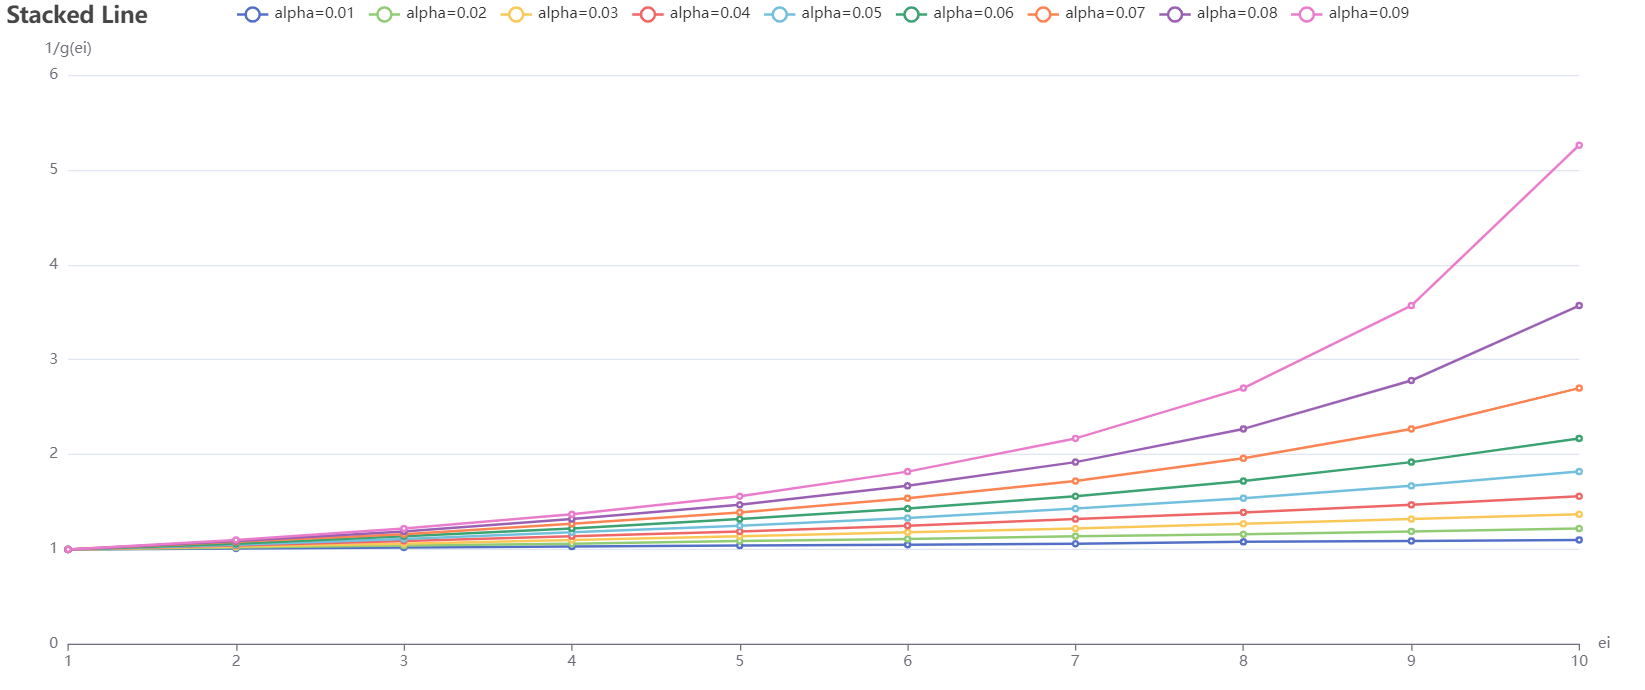
\includegraphics[width=0.9\textwidth]{Stacked Line.png}
        \caption{Relationship between $\cfrac{1}{g(e_i)}$ and $e_i$}
        \label{line}
    \end{figure}
    \textbf{Definition (\textit{Load})} The \textit{load $L_i$} of each core \textit{i} is the total processing \textbf{time} of all job blocks executing on it. \\
    
    \textbf{Observation} The decay factor $\alpha$ of executing speed can have a great influence on the executing time, so we must consider the number of cores we assign to a job with $\alpha$. Here we list the relationship between $\alpha$, the number of cores we assign to a job and the executing speed. \\
    
    
    
    \textbf{Single-Core Algorithm (\textit{Greedy Algorithm Version})} Based on the observation,we design a greedy algorithm to assign each job one single core. First, we sort the jobs by their processing time on a single core from long to short.Then we assign jobs by order. Each time we assign a job, the algorithm chooses the core whose current load is smallest.
    
    \begin{center}
        \begin{minipage}{15cm}
        \begin{algorithm}[H]
            \SetAlgoLined
            \KwIn{n,m,$\alpha$,S,size,b}
            \KwOut{$L^* = max_job_i tf(job_i)$}
            jobTime[] $\leftarrow$ 0 \; \tcp{every job's execution time}
            idx[i] $\leftarrow i$\; \tcp{record every job's executing order}
            \For{j $\leftarrow$ 0 \KwTo m-1}{
                cmp[j].amt $\leftarrow$ 0 \; \tcp{A struct to store the information of core;amt is current load}
                cmp[j].id $\leftarrow$ j \;
                push cmp[j] to CoreQueue \; \tcc{A minimal priority queue to get the core whose current load is smallest}
            }
            \For{$i\leftarrow 0$ \KwTo $n-1$}{
                $jobTime[i] \leftarrow (\sum_b^i size(b_j^i)/s_i)$\;
            }
            Sort jobTime[idx[i]] with decreasing order\; 
            \For{$i \leftarrow 0$ \KwTo $n-1$}{
                $cmptemp \leftarrow CoreQueue.pop()$\;
                $cmptemp.amt += jobTime[idx[i]]$\;
                $CoreQueue.push(cmptemp)$\;
            }
            $L_* \leftarrow max_{core_j} cmp.amt$\;
            

        \caption{Single-host: Greedy Algorithm Version}
        \end{algorithm}
        \end{minipage} 
        \end{center}
    
\subsubsection{Algorithm Analysis}
    \textbf{Time complexity:} Main time cost of our algorithm goes to sorting the n-size array \textit{jobTime} and reorganization of priority queue \textit{CoreQueue} after each pop and push. Sorting's time complexity is \textit{O($n \log n$)}. In the n-times \textit{for-loop}, each push's and pop's time complexity is \textit{O($\log m$)}. So the total time complexity is \textit{O($n \log n + (n + m) \log m$)}.
    
    \textbf{Approximation Rate}
    
    Let's now analyze the approximation rate in the manner described in the  textbook \cite{10.5555/1051910}.
    
    Denote $t_j$ as the time consumes by the jth largest job. So, $t_1 \geq t_2 \geq \cdots t_n$. The  processing time is T.
    
    \textit{Lemma 1:} The optimal processing time $T^*$ is at least $\frac{1}{m}\sum_j tp^j$.
    \begin{equation}
        T^* \geq \frac{1}{m}\sum_j tp^j
    \end{equation}
    
    \textit{Proof:} Suppose at the best situation, the job can scatter evenly on all the cores, then we know that the OPT must be greater than this. Therefore, $T^* \geq \frac{1}{m} \sum_j tp^j$.
    
    
    \textit{Favourable Situation:} In the Favourable Situation, the most heavily loaded core ends up with more than 1 job. We can show here that under this situation, our approximation rate is of constant level.
    
    \textit{Proof:} Denote i as the slowest core index, and k is the last job placed on the core i, which consumes $t_k$ time. Because there is more than 1 job on core i, and the scheduling process follows the order from big to small, $k \geq m+1$.
    Denote $T_j$ as the total workload. We have that $T_i - t_k \neq 0$ is smaller than all the other cores' workload at that time, therefore, $m(T_i - t_k) + t_k \leq \sum_j tp^j$. 
    \begin{equation}
        \begin{aligned}
            &T^* \geq \frac{1}{m}\sum_j tp^j\\
            &T^* \geq \frac{1}{m}\sum_j t_j\\
            &T^* \geq(T_i - t_k) + \frac{1}{m} t_k \\
            &T^* \geq T_i -  \frac{m-1}{m} t_k \\
            &T^* \geq T_i -  \frac{m-1}{m} t_{m+1},\ k\leq m+1 \\
        \end{aligned}
        \label{pre 1.3.1.1}
    \end{equation}
    
    Under this circumstances, we shall also notice the following property.
    \begin{equation}
        \begin{aligned}
            &T^* \geq \frac{1}{m}\sum_j t_j\\
            &T^* \geq \frac{1}{m}(t_1 + \cdots + t_{m+1})\\
            &T^* \geq \frac{m+1}{m}t_{m+1}\\
        \end{aligned}
        \label{pre 1.3.1.2}
    \end{equation}
    
    Based on Equation \ref{pre 1.3.1.1} and \ref{pre 1.3.1.2}, we can have below property.
    \begin{equation}
        \begin{aligned}
            &T_i \leq T^* +  \frac{m-1}{m} t_{m+1}\\
            &T_i \leq T^* +  \frac{m-1}{m} \cdot \frac{m}{m+1} T^*\\
            &T_i \leq  \frac{2m}{m+1} T^*\\
            &T_i \leq  (2-\frac{2}{m+1}) T^*\\
        \end{aligned}
        \label{approx1}
    \end{equation}
    
    The approximation rate of $(2-\frac{2}{m+1})$ is actually a rather tight bound for the \textit{Favourable Situation}. So we prove here that when the last core has loaded at least 2 jobs, our approximation is very appealing.
    
    
    \textit{Bad Situation:} In the bad situation, where the slowest core ends up with only one job on it, however, can be arbitrarily bad. 
    
    \textit{Proof:} This is quite obvious there is one job that should originally split into small pieces is only assigned one core and lagged behind.\\
    
    \textbf{Modification} In most cases,our algorithm has the approximation rate exactly smaller than 2. However, as is mentioned before, there is bad cases that make our algorithm dumpy. According to our algorithm, every job is assigned to one single core. A single extremely large job with a handful data blocks can be catastrophic. So we do need some improvement of our algorithm to approach some extreme cases.
    
    After the assignment of jobs to cores by our greedy algorithm, we judge the number of jobs on the core who has the maximum load. If the jobs number is 1, it means there exists an extremely large job, then we may need to change our algorithm to more advanced ones (talked about and analyzed in Problem 2). 
    
\subsection{Results and Discussions}
    \label{simplified analysis}
    In the previous analysis, we've already discussed that there are 2 situations for the single-core strategy greedy approximation.
    
    \subsubsection{Favourable Cases}
    The first situation is relatively good. There are lots of jobs, and their sizes are evenly distributed.
    It can be seen as a favourable case for our algorithm. We have a constant approximation rate, as discussed before. So let's visualize our results in these cases. Figure \ref{single-host-good} shows our results on the test file of $task1_case1.txt$ given by TAs. In this example, all the jobs sizes are distributed evenly, and thus yields a really good result. Just as we have proved before, in such cases the approximation rate is appealing.
    
    \begin{figure}[H]
        \centering
        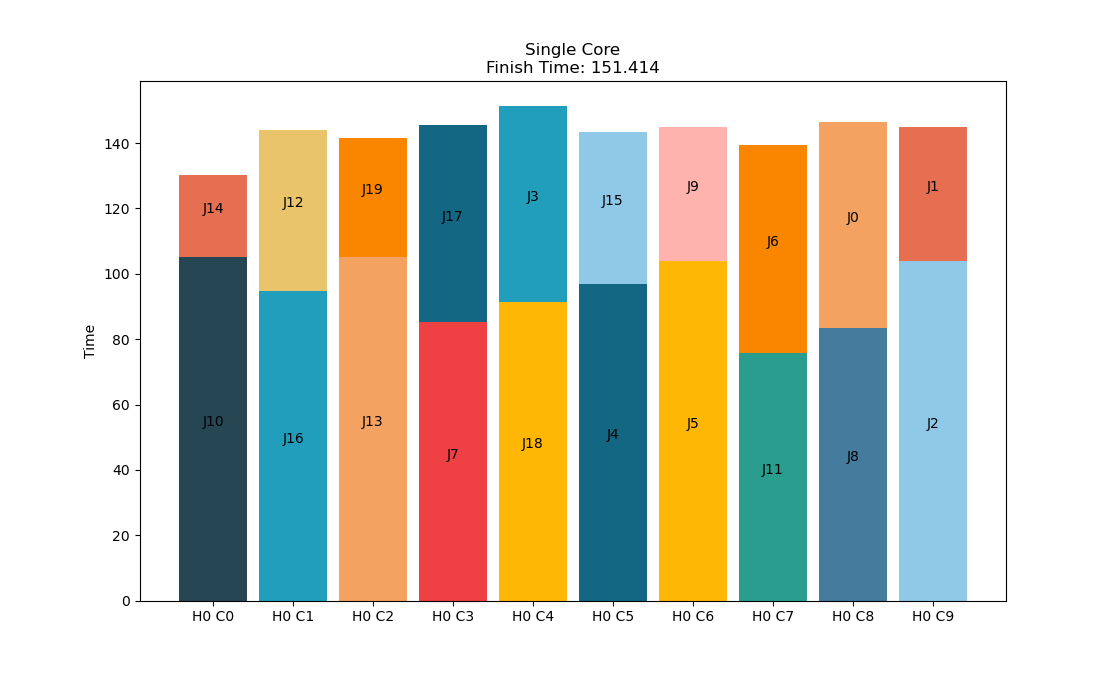
\includegraphics[width = 350pt]{single-host-good.png}
        \caption{Single Host Greedy Approximation}
        \label{single-host-good}
    \end{figure}
    
    The CPU utilization rate in this example is 95\%, which means the approximation rate is close to 1, if this is not the OPT.

    \subsubsection{Bad Cases}
    In these cases, either the job number is small, even smaller than the number of cores, or the job sizes are biased. In these cases, we have a common problem that there are jobs that should originally be split up still maintained on a same core, which deteriorate the performance by large. We can see the bad performance below, in Figure \ref{single-host-bad}. This is the toy example displayed in .pdf given to us.
    
    \begin{figure}[H]
        \centering
        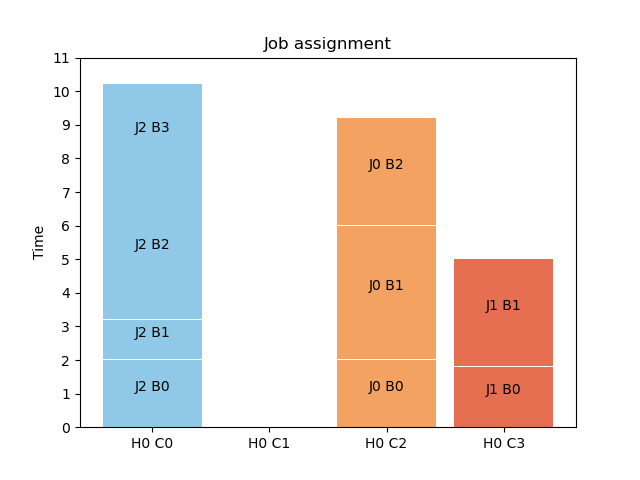
\includegraphics[width = 250 pt]{single-host-bad.png}
        \caption{Single Host Bad Example}
        \label{single-host-bad}
    \end{figure}

We can see here that this is definitely not a reasonable assignment. Actually we will revisit this problem again with our advanced algorithm we developed in the Comprehensive Version below. You can refer to Section \ref{comprehensive analysis} for more details on how we deal with this bad problem for our current simple greedy approximation.

\subsubsection{A Little Conclusion}
In Problem 1, we prove that the simplified version is already a NPH problem, so a polynomial time solution is not likely to be possible. Therefore, we introduced the greedy approximation algorithm, and displayed the results as before. There are some cases that our simple greedy approximation algorithm goes bad. Let's see the Comprehensive Version Problem and our advanced algorithm.

\section{A Comprehensive Version among Multiple Hosts}
    In this problem, we need to consider the possibility of transferring the blocks to other hosts to speed up calculation. At the same time, there exists the transmission cost. This problem is even harder that it is NP-hard problem. We will give the formalization, NP-hard proof, algorithm(greedy and random walk) and results.
\subsection{Formalization of the problem}
    Based on the former formalization of the problem, we give the formalization of scheduling program with multiple hosts.
   \subsubsection{Input}
    First, we will formalize the input as
    \begin{center}
            \textit{Input = (J,B,$\widetilde{B}$,C,$\alpha$,N,S,size)},
    \end{center}
    
    in which $J=\{ job_0,job_1,\cdots,job_{n-1}\}$ represents the jobs, $B_{lj}^i$ represents the set of data blocks of job \textit{i} allocated to core $c_j$, $\widetilde{B_{lj}^i}$ represents the set of data blocks of $job_i$ allocated to core $c_j^l$ but not initially stored on $h_l$ , $B^i$ represents the set of data blocks of job \textit{i}, $C_i=\{ c_0^i,c_1^i,\cdots,c_{m_i-1}^i\}$ represents the cores on host \textit{i}, $0 < \alpha < 1$ represents the decay factor in function $g(e_i) = 1 - \alpha(e_i - 1)$, $N=\{n_0,n_1,\cdots,n_{n-1}\}$ represents the numbers of data blocks in each job, $S=\{s_0,s_1,\cdots,s_n\}$ represents the calculation speed of each job on one single core and \textit{size} is the function to fetch the size of data blocks.
    
    \subsubsection{Output}
        Second, we will formalize the output, namely the scheduling scheme, as
        
        \begin{center}
            $Sol = \{T,Core\}$,
        \end{center}
        
    in which, $T_i=\{t_0^i,t_1^i,\cdots,t_{|B^i|-1}^i\}$ represents each job \textit{i}'s block's starting time, \\  $Core_i = \{Core^i_0,Core^i_1,\cdots,Core^i_{|B^i|}\}$ and $Core^i_k$ represents the core ID on which $i$-th job's $k$-th block runs. With the starting time and core allocation scheme, we can easily calculate everything we want.
    
        \subsubsection{Objective Function and Constrains}
        Third, we will formalize the calculation process, objective function and the constrains. The processing time and finishing time of $job_i$ on core \textit{j} of host \textit{l} are
        
        \begin{center}
        $$
        \begin{aligned}
            tp^i_{lj} &= \cfrac{\sum_{b^i_k \in B^i_{lj}} size(b^i_k)}{s_i \cdot g(e_i)}+\cfrac{\sum_{b^i_k \in \widetilde{B^i_{lj}}} size(b^i_k)}{s_t}\\
            tf^i_{lj} &= t_i + tp^i_{lj}
        \end{aligned}
        $$
        \end{center}
        
        Therefore the finishing time of  core $c_j^l$ for $job_i$ is
        
        \begin{center}
        $$
        \begin{aligned}
        tf(job_i) &= \max_{c_j^l} tf^i_{lj}\text{, for } c_j^l \in C
        \end{aligned}
        $$
        \end{center}
        
        With all the definitions above, we can give the objective function
        
        \begin{center}
            $\min \max_{job_i} tf(job_i)\text{, for } job_i \in J$.
        \end{center}
        
        And the constrains are as follows.
        \vspace{-5mm}
        \begin{center}
        $$
        \begin{aligned}
            \forall i, j \in J,
            (i \neq j) \wedge\left(A_{i} \cap A_{j} \neq \phi\right)
            \rightarrow 
            t_{i} \geqslant t f\left(job_{j}\right) \vee t_{j} \geqslant t f\left(job_{i}\right)
        \end{aligned}
        $$
        \end{center}
        
        $A_i$ is the set of cores assigned to i-th job. This constrain means that if any two jobs are allocated the same core, then the time of starting of one job can not be smaller the time of ending of the other job.
    

    
\subsection{NP-Hardness of the Comprehensive Version}
\subsubsection{NPH Proof by restriction}
We still use the simple proof by restriction to prove the NP-hardness of the Comprehensive Version.

\textbf{Cook Reducibility:} The Simplified Version can be solved by calling the oracle of the Comprehensive Version by restricting (host) q=1, and all the data blocks are on the very single core. Therefore, the Simplified Version can be polynomial time reduced to the Comprehensive Version. 
\begin{equation}
    Simplified\ Version\leq_p Comprehensive\ Version
\end{equation}

The simplified version is NPH as we've proved before in Section \ref{NPH1}, so the comprehensive version is NPH.

\begin{equation}
    Comprehensive\ Version \in NPH
\end{equation}

\subsubsection{Beyond NPC}
Just as what we've proved in Section \ref{NPH1}, the Comprehensive Version is beyond NPC if $co-NP \neq NP$. The details are memtioned before.
\begin{equation}
    co-NP \neq NP \Longrightarrow Comprehensive\ Version \notin NP
\end{equation}

\subsection{Algorithm Design and analysis}
    \textbf{Redefinition(\textit{Load})} In our multi-host version, the load $L_i$ of one core \textit{i} is the total transmission time plus the processing time of the job blocks.\\
    
    \textbf{Assumption} In real life case, the transmission speed through Internet can largely exceed the processing speed of jobs. So in our multi-host version, we make a similar assumption that transmission speed exceeds processing speed(e.g. ten times faster).\\
    
    \subsubsection{Multi-host Algorithm 1 (\textit{Simple One-Core Greedy Algorithm})} According to the assumption, the transmission time has a smaller impact on the executing time. So when considering this problem, we can temporarily ignore the transmission progress and pay more attention to the processing progress. Then the multi-host problem can be degraded into a similar problem to single core problem. So our Algorithm 1 takes the same idea. We sort jobs by their single core processing time and assign them one single core to run. Each time we assign a job, we choose the core whose current load is smallest and then transmit all the blocks of the job to the core to run.\\
    
        \begin{center}
        \begin{minipage}{15cm}
        \begin{algorithm}[H]
            \SetAlgoLined
            \KwIn{n,m,q,$\alpha$,S,size,B,C,b,$s_t$}
            \KwOut{$L^* = max_job_i tf(job_i)$}
            jobTime[] $\leftarrow$ 0 \; \tcp{every job's execution time}
            idx[i] $\leftarrow i$\; \tcp{record every job's executing order}
	 \For{i $\leftarrow$ 0 \KwTo q-1} {
            	\For{j $\leftarrow$ 0 \KwTo m[i]}{
               		 cmp.amt $\leftarrow$ 0 \;
            	  	  cmp.id $\leftarrow$ j \;
			 cmp.idh $\leftarrow$ i \;		\tcp{cmp is a struct to store information of cores }
              	 	 push cmp to CoreQueue \; \tcc{A minimal priority queue to get the core whose current load is smallest}
		}
            }
            \For{$i\leftarrow 0$ \KwTo $n-1$}{
                $jobTime[i] \leftarrow (\sum_b^i size(b_j^i)/s_i)$\;
            }
            Sort n jobs by their jobTime so that jobTime[idx[0]] $\geq$ jobTime[idx[1]] $\geq$ ... $\geq$ jobTime[idx[n-1]]\; 
            \For{$i \leftarrow 0$ \KwTo $n-1$}{
                    $cmptemp \leftarrow CoreQueue.pop()$\;
	                $ hid \leftarrow cmptemp.idh $\;
	                $ cid \leftarrow cmptemp.id $\;
	        	\For{$j \leftarrow 0$ \KwTo $|B^i|$} {
	                \uIf{$b_j^i \in B_{hid,cid}^i$}{
	                $ cmptemp.amt +=size(b_j^i)/s_i $\; 
	                }
	                \Else{
	                $ cmptemp.amt += size(b_j^i)/s_i +size(b_j^i)/s_t$\;
	                }
                 }
                     $CoreQueue.push(cmptemp)$\;
            }
            $L_* \leftarrow max_{core_j} cmp.amt$\;
            

        \caption{Multi-host: Greedy Algorithm Version}
        \end{algorithm}
        \end{minipage} 
        \end{center}
    
    \textbf{Time complexity:} The main time cost of our algorithm goes to the sorting of the n-size array \textit{jobTime}, pop and push action of the priority queue \textit{CoreQueue} in the for-loop. The sorting's time complexity is \textit{O($n \log n$)}. The pop and push cost \textit{O($\log m$)} in the n-times for-loop. So the total time complexity is  \textit{O($n \log n + (n + m)\log m$)}.\\
    
    \subsubsection{Multi-host Algorithm 2 (\textit{SLS + Greedy Approximation + Random Walk})}  
    In order to search the feasible solution space with a better coverage, we can turn to heuristic algorithms. A very appealing method applied in many fields is the \textbf{Stochastic Greedy Local Search} with or without the reinforcement of the \textbf{Random Walk} \cite{DECHTER2003191}. Here, we try to implement this idea on our problem.
    
    \textbf{A local search algorithm} starts from a randomly chosen complete instantiation and moves from one complete instantiation to the next. The search is guided by some cost function related to the task, and at each step the value of the variable that leads to the greatest reduction of the cost function is changed. Then the algorithm may be restarted from a different initial random assignment. The algorithm stops either when the cost is minimized or when when there is no way to improve the current assignment by changing one variable. \\
    
    To reduce the chance of reaching a local minimum, when randomizing the elements, we use another technique \textbf{Random Walk}. Random Walk starts with a random assignment and randomly flip the value of its variables.\\
    
    \textbf{Definition(\textit{Solution Space})} The Solution Space of our algorithm denotes the order jobs executing and the numbers of cores assigned to the jobs. Typically, it's a struct Sol \{vector$<$int$>$ order, vector$<$int$>$ core\_num \}. \\
    
    \textbf{Definition(\textit{flip})} A \textbf{flip} is an action of swapping two neighbouring jobs' executing order or a increase/decrease of the number of cores assigned to one job. A flip causes a local change in out Solution Space.\\
    
    Then we can get our \textbf{Multi-host Algorithm 2}. For \textit{MAX\_TRY} times, we randomly produce a Solution Space, and in every Solution Space, we do \textit{MAX\_FLIP} times of actions. Each action has two choices. The first choice, with probability \textit{p} to be chosen, does a flip. And the other, with probability \textit{1-p}, does a random walk. In our algorithm, the random walk simply takes no action, namely avoid doing a flip. \\
    
    In each step, given the Solution Space, namely we know the order jobs should execute and the number of cores assigned to jobs. The problem is degraded into several sub-problems of minimizing the executing time of jobs. Here we use Greedy Algorithm. For a certain job \textit{j} which is assigned \textit{k} cores, we find \textit{k} cores which has the \textit{k} smallest load of all cores. Since each block of the same job has the same processing speed, the size of block is proportional to processing time. So we sort blocks of the same job from big size to small size. And each time we assign a block to a core, we choose the core which has the smallest current load in the selected \textit{k} cores.
    
        \begin{center}
        \begin{minipage}{15cm}
        \begin{algorithm}[H]
            \SetAlgoLined
            \KwIn{n,m,q,$\alpha$,S,size,B,C,b,$s_t$}
            \KwOut{$L^* = max_job_i tf(job_i)$}
            blockTime[] $\leftarrow$ 0,idx[i] $\leftarrow i$ \; 

    	 \For{i $\leftarrow$ 0 \KwTo q-1} {
                \For{j $\leftarrow$ 0 \KwTo m[i]}{
                   	cmp.amt $\leftarrow$ 0,cmp.id $\leftarrow$ j,cmp.idh $\leftarrow$ i \;
    			    \tcp{cmp is a struct to store information of cores }
                  	push cmp to CoreQueue \;
                  	\tcc{A minimal priority queue on current workload}
    		    }
        }

	\Repeat{repeat $MAX\_TRY$ times}{
	    randomly initialize sol\;
		\tcp{Greedy Algorithm to solve sub-problem }	
		\ForAll{job}{
			normalize job's execution time\;
			sort blockTime[idx[i]] to decreasing order \;
			pick next job and update core time in queue \;
		}
		
		\tcp{Greedy Search: take  flips}
		\Repeat{repeat  $MAX\_FLIP$ times}
		{randomly yield a choice for order or core number\;
			\uIf{change order} {
				randomly change two near job's order\;
				calculate the time cost\;
				randomly choose to become better or not\;
			}
			\ElseIf{core number}{
				randomly change the core number of a job\;
				calculate the time cost\;
				randomly choose to become better or not\;
			}
		}

		
	}

        \caption{Multi-host: Greedy Algorithm+Greedy Search+Random Walk Version}
        \end{algorithm}
        \end{minipage} 
        \end{center}
    
    \textbf{Time complexity: } In the \textit{MAX\_TRY}-times for-loop, each time we need to use greedy algorithm to solve the sub-problem like \textbf{Algorithm 1} and \textbf{Algorithm 2}, this step's time complexity can be analyzed similarly: for each job \textit{i}, it needs \textit{O($|B^i| \log |B^i|$)} to sort and \textit{O($(|B^i|+e_i) \log e_i$)} to do priority queue's work, so this step's time complexity is \textit{O($n \cdot \max_i (|B^i| \log |B^i|)$)}. Then in the \textit{MAX\_FLIP}-times for-loop, local change will lead to another computation of the sub-problem. So in total, the time complexity is \textit{O($ n \cdot MAX\_TRY \cdot MAX\_FLIP \cdot  \max_i (|B^i| \log |B^i|)$)}.
    
\subsection{Results and Discussions}
    \label{comprehensive analysis}
\subsubsection{Comparison between Simple Greedy and SLS + Random Walk}
    \textbf{Differences:} For our Simple Greedy Algorithm, each job can only be assigned to a single core, which can be problematic though it escapes decay factors and may or may not avoid transmission overhead. On the other hand, SLS + Random Walk allows random issues (more like a NTM), for which reason it can cover a much larger region in our feasible space. It searches for local optimum  solution in local regions and search for global optimum by random initialization. Thus, in SLS + Walk algorithm, we can optimize multi-core assignments, that is, a single job can be put on different cores to run. This is  the major difference.
    
    \textbf{Common Points:} 
    The common point is that all our algorithm didn't take transmission speed into account when scheduling, which may or may not deteriorate the performance of our algorithm to some extent. On other aspects, our algorithm possess a solid theoretical foundation.
    
    \textbf{Case 1: Simple Greedy performs better}
    
    There are some cases when simple single-core processor Greedy Algorithm performs better than our SLS + Walk, in which cases, jobs are distributed evenly, or in another words, the \textit{Favourable Cases} in Section \ref{simplified analysis}. Why? It's because that in single-core Simple Greedy Approximation, the decay factor problem is reduced to the minimum scale, while SLS + Walk suffers.
    
    Here goes our example, the  \textit{Favourable Cases} in Section \ref{simplified analysis}. The following is the SLS + Walk result, where 217s is larger than 151s shown in Figure \ref{single-host-good}. Compare Figure \ref{single-host-good} and Figure \ref{sigle-host-SLS}.
    
    \begin{figure}[H]
        \centering
        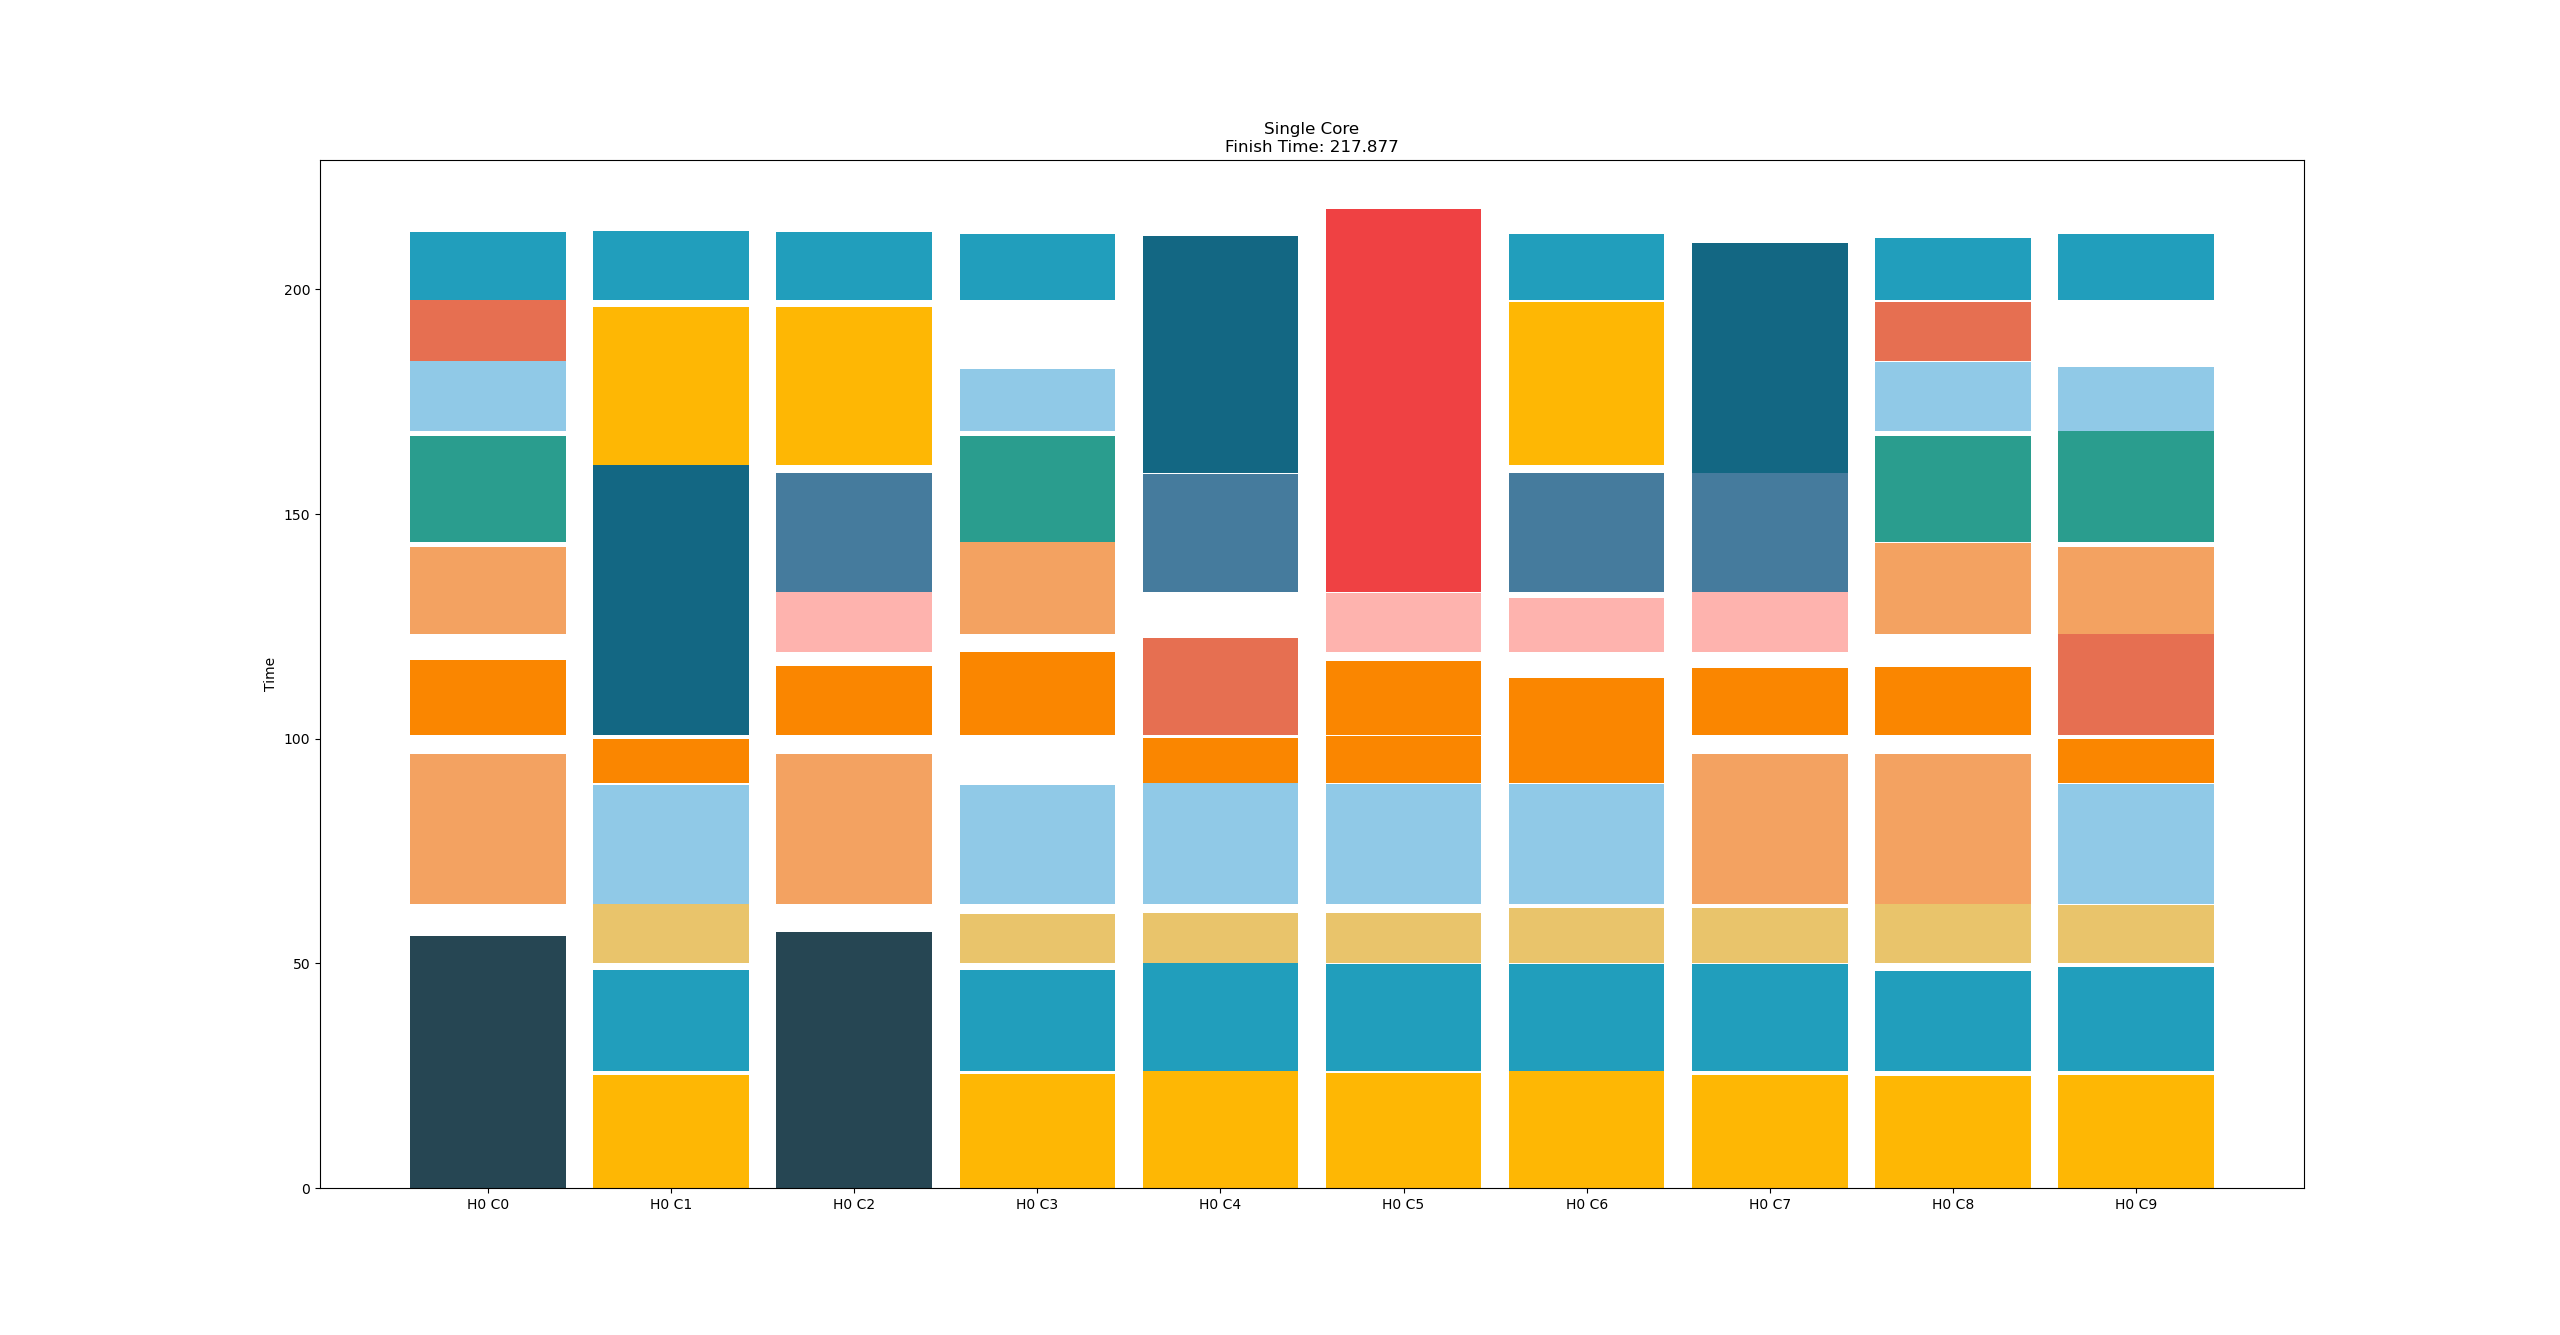
\includegraphics[width = 400pt]{sigle-host-SLS.png}
        \caption{SLS + Walk Scheduling}
        \label{sigle-host-SLS}
    \end{figure}
    
    We can actually find out in the so-called \textit{Favourable Cases}  Simple Greedy Algorithm outperforms our SLS + Walk.
    
    
    \textbf{Case 2: Other Cases Where SLS + Walk Stands Out}
    
    Actually, in virtually all the other cases, SLS + Walk gives out a far more reasonable answer than that given out by the Simple Greedy Algorithm. Let's first see some small cases.
    
    The first example is the toy example in the .pdf, the single-host version, also refer to Figuer \ref{single-host-bad} we've discussed before. In the Figure \ref{single-host-COM}, we can see that the SLS + Walk successfully solved the previously so-called \textit{Bad Cases}. By permuting all possible combination, we can also find that our SLS + Walk actually gives out OPT in this case.
    
    \begin{figure}[H]
        \centering
        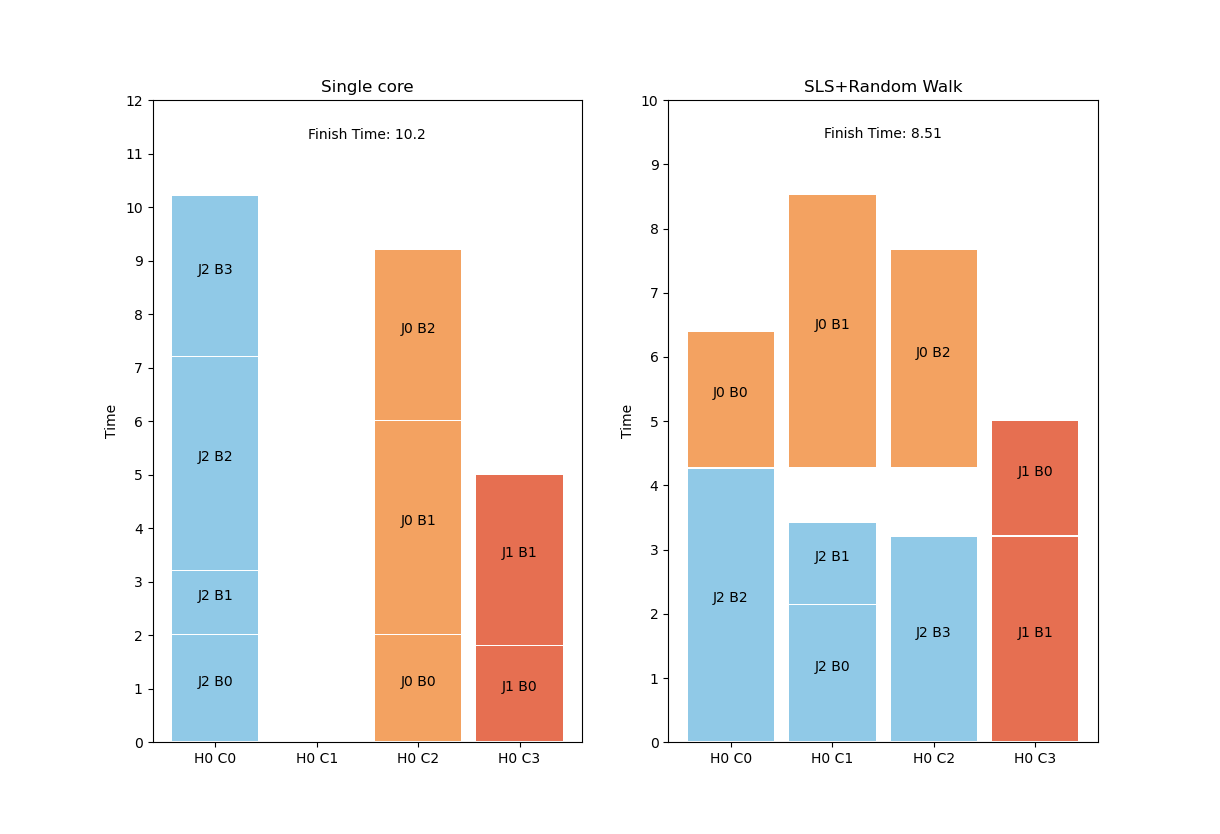
\includegraphics[width = 400pt]{single-host-COM.png}
        \caption{Single-Core Comparison}
        \label{single-host-COM}
    \end{figure}
    
    Let's see also the multi-host toy example given in the .pdf. In Figure \ref{multi-host-SIM-COM}, we can see that SLS + Walk again solves the \textit{Bad Cases} astonishingly. Our SLS + Random Walk performs outstandingly here.
    
    \begin{figure}[H]
        \centering
        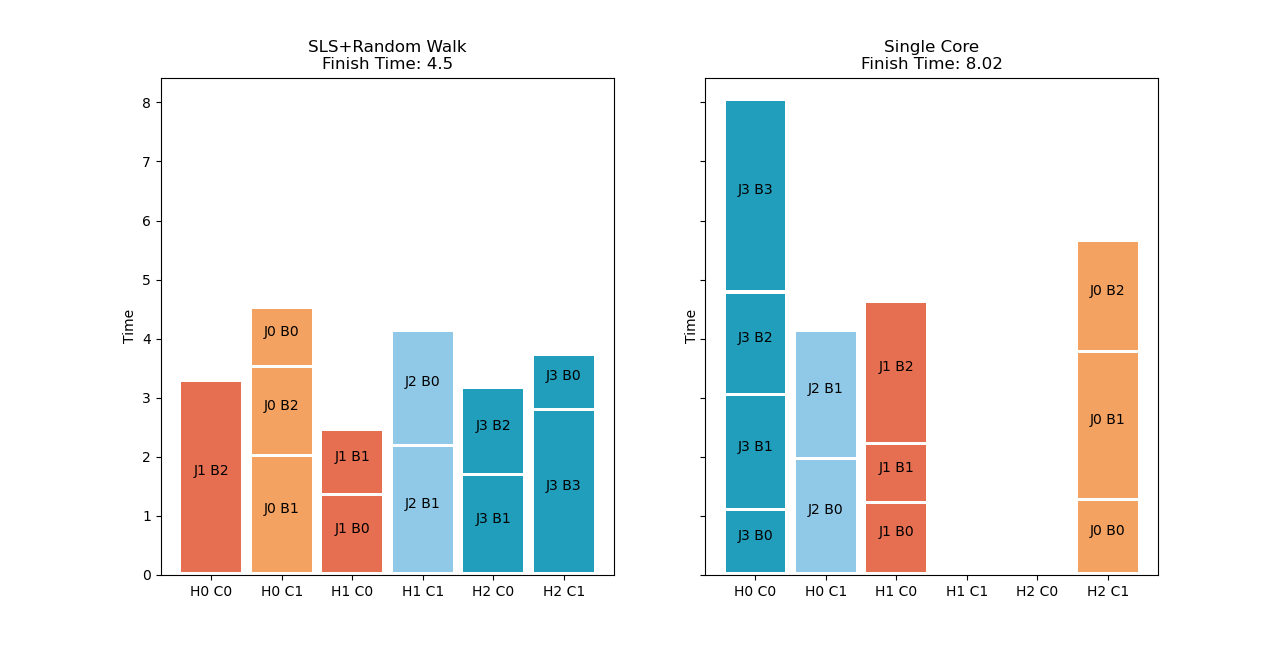
\includegraphics[width = 400pt]{multi-host-SIM-COM.png}
        \caption{Scheduling upon Multi-Host Simple Problem}
        \label{multi-host-SIM-COM}
    \end{figure}
    
    Let's see the final example for this section. This is the test problem in "test2\_case2.txt" given by our adorable TAs. In Figure \ref{multi-host-COM}, we can see that SLS + Walk again performs really good. For Simple Greedy, it can never resolve such problems that involve enormous job with a handful of data blocks. Here, SLS + Walk reinforce it! 
    
    \begin{figure}[H]
        \centering
        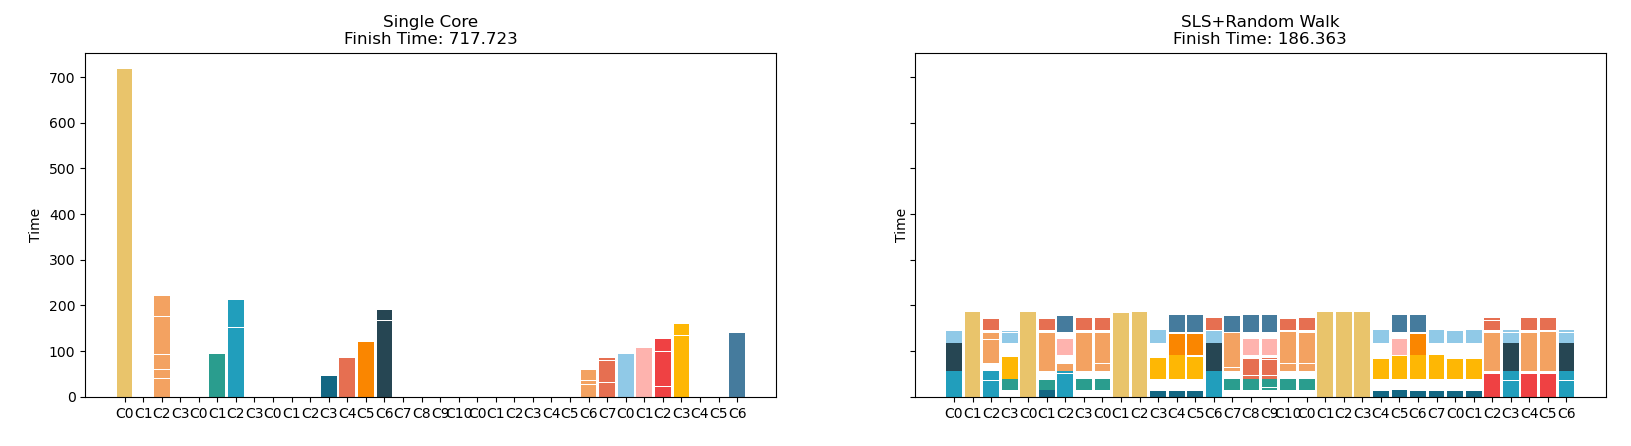
\includegraphics[width = 420pt]{multi-host-COM.png}
        \caption{Scheduling upon Multi-Host Complicated Problem}
        \label{multi-host-COM}
    \end{figure}
    
    186s is significantly better than 717.7s.
    
\subsubsection{Further Analysis for SLS + Walk}
    \textbf{Case 3: Performance Issue for Large Cases}
    
    In these large cases, we have mountainous jobs to finish, each with dozens of blocks, and accordingly, we have even more hosts and cores that is handy to use.
    
    Let's do some experiments on SLS + Random Walk to observe the results on large cases.
    
    The following Table \ref{LargeCases} contains the comparison and the key performance issue of communication decay and CPU utilization rate. This Table can give us some idea of the scalability of our algorithms.
    
% Please add the following required packages to your document preamble:
% \usepackage{multirow}
\begin{table}[H]
\begin{tabular}{ccccccc}
\hline
                        &                 & 1        & 2        & 3        & 4        & 5        \\ \hline
\multirow{2}{*}{simple   greedy} & utilization rate         & 0.15     & 0.97     & 0.37     & 0.27     & 0.34     \\
                                 & efficacious running time & 14087    & 257      & 170      & 276      & 51       \\ \hline
\multirow{3}{*}{SLS   + Walk}    & utilization rate         & 0.75     & 1        & 0.77     & 0.82     & 0.75     \\
                                 & efficacious running time & 16050    & 259      & 177      & 300      & 53       \\
                                 & decay penalty rate       & 1.139348 & 1.007782 & 1.041176 & 1.086957 & 1.039216 \\ \hline
\multicolumn{1}{l}{}             & \multicolumn{1}{l}{}     & 6        & 7        & 8        & 9        & 10       \\ \hline
\multirow{2}{*}{simple   greedy} & utilization rate         & 0.12     & 0.19     & 0.15     & 0.07     & 0.21     \\
                                 & efficacious running time & 82913    & 67876    & 80907    & 49239    & 74798    \\ \hline
\multirow{3}{*}{SLS   + Walk}    & utilization rate         & 0.57     & 0.78     & 0.7      & 0.53     & 0.75     \\
                                 & efficacious running time & 86949    & 112700   & 100282   & 64645    & 106353   \\
                                 & decay penalty rate       & 1.048678 & 1.660381 & 1.239472 & 1.312882 & 1.42187  \\ \hline
                                 \label{LargeCases}
\end{tabular}
\caption{small and large cases}
        
\end{table}
    
    We can tell from here that SLS + Walk can almost always have a good CPU utilization Rate, which is always welcomed. Besides, we can see from each cases, the decay rate, that is, the extra amount of work one must suffer from the benefit of more task-level parallelism. However, we can see that, almost always, the benefit from CPU utilization rate outweighs the overhead of decay rate.
    
    Finally, we generate a massive example with hundred of jobs, thousands of blocks. We can take it as an extreme case, in Table \ref{ExtremeCase}.
    
    \begin{table}[H]
    \centering
\begin{tabular}{ccc}

\hline
                       &                 & 11      \\ \hline
\multirow{2}{*}{simple   greedy} & utilization rate         & 0.99    \\
                                 & efficacious running time & 1965194 \\ \hline
\multirow{3}{*}{SLS   + Walk}    & utilization rate         & /       \\
                                 & efficacious running time & /       \\
                                 & decay penalty rate       & /       \\ \hline
                \label{ExtremeCase}
\end{tabular}
\caption{Extreme Case} 
\end{table}
    
    In such an extreme example, our SLS + Walk ceased to work because of the time complexity. However, our Simple Greedy loves it, whose CPU utilization rate is 99\%, almost OPT.
    
    Now we have a more comprehensive overview upon the performance of our Simple Greedy Algorithm and SLS + Random Walk Algorithm.
    
    \textbf{Case 4: Transmission Rate and Decay Factor Matters}
    
    What if the transmission overhead is large that cannot be overlooked in scheduling processes? This is also a key issue we shall experiment on.
    
    We actually observed that all the 3 algorithms perform worse than ever when transmission speed is unfavourable, because none of them have taken it into account. Figure \ref{Case4} can gives us some hints on it.
    
    \begin{figure}[H]
        \centering
        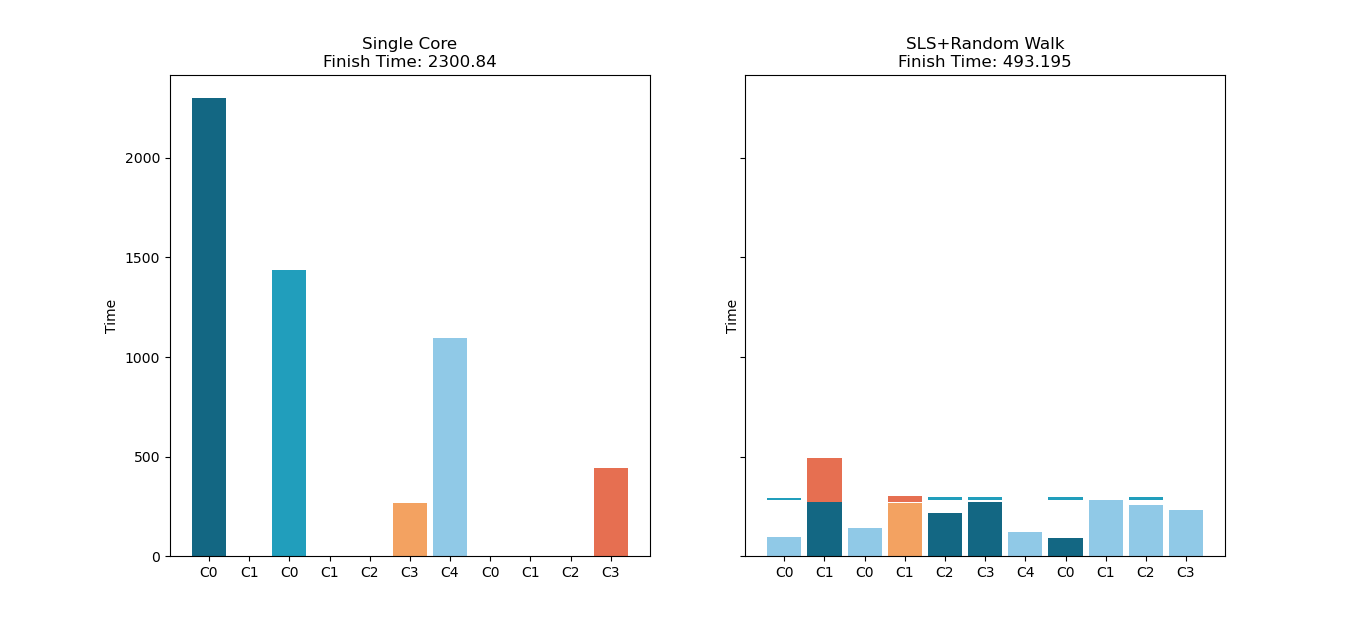
\includegraphics[width =350pt]{Case4.png}
        \caption{Large Transmission Overhead}
        \label{Case4}
    \end{figure}
        
    In modern Hadoop, if the transmission bandwidth is enough, then this problem will never occur. That's why we aim to improve transmission bandwidth.
    
    Anyway, taking into account the transmission speed is a possible improving field for future researches. 
    
\subsubsection{A Little Reflection}
We can see that in most cases, SLS + Random Walk Algorithm performs astoundingly well. That's why we introduced this algorithm in our project report.
    
\section{Conclusion}
To sum up, our Simple Greedy Algorithm performs well for some \textit{Favourable Cases} while the data blocks are distributed evenly. However, the performance of this trivial algorithm can degrade heavily when some \textit{Bad Cases} happen.

To compare with it, when the decay factor is not too large, no matter how the data blocks or cores on hosts distribute, our SLS + Walk algorithm can always give a pretty good result which is a very close approximation of the optimal solution, since the algorithm can nearly traverse through the feasible solution space.  

However, the decay factor and big-size data can challenge our SLS + Random Walk Algorithm a lot. From our analyzed time complexity, \textit{MAX\_TRY} and \textit{MAX\_FLIP} influence the performance a lot. With larger randomization iteration times, we may get better results, but the time cost goes up. Moreover, with larger decay factor, the performance of parallel processing suffers a lot and sequential running is better.

From the analysis above, it hinds on us that in real world, when handling similar load-balancing problem or resource scheduling in distributed system, we should take factors like transmission time and processing speed decay when doing parallel computing into consideration, which may influence a lot to our decision whether parallel computing is better. And the trade-off between time complexity and performance is another question we must consider.

Last but not least, there isn't a cure-all algorithm for this problem in the foreseeable future. However, the basic concept of greedy approximation and random/heuristic algorithm is always an option to us for an acceptable good solution.
    
\section{Acknowledgements}    
    In writing this paper, we have benefited from the presence of our teacher and our classmates a lot. They generously helped us figure out some hard problems and made many invaluable suggestions. We hereby extend out grateful thanks for their kind help, without which the paper would not have been what it is.
    
    To be honest, the beginning is the most difficult. Because there is not a clear direction, we tried many possible ways but all failed. Later, we just jumped out of the limitation of the methods that we had already learnt, tried to learn some new methods to solve the problem. And that how we come up these fascinating algorithm. We have to admit that the most powerful algorithm sometimes comes from simple ideas, like the random walk algorithm and greedy search algorithm. Also, we learnt how to analyse the approximation rate and the NP related problem. In sum, we really benefited a lot from this project.
    
    As for suggestions, we hope that there could be some useful reference or possible methods to solve the problem, otherwise we really have to spend a lot of time on designing the algorithm. It feels bad when an algorithm doesn't work. But the designing process and see the excellent output is really attractive.
    
    Thank you very much! Let it be our ending.

\section{Appendix}
\begin{appendices}

\begin{table}[htbp]
\caption{Symbols and Definitions}
\begin{center}
\begin{tabular}{c|c}
\toprule
\textbf{Symbols} &\textbf{Definitions}  \\
\midrule
$n$ & The number of jobs  \\ 
$m$ & The number of cores \\
$q$ & The number of hosts  \\ 
$A_i$ & The set of cores assigned to i-th job  \\
$job_i$, $J$ & $job_i$ is the $i$-th job. The job set is $J=\{job_0, \cdots, job_{n-1}\}$. \\ 
$h_l$, $H$ & $h_l$ is the $l$-th  host. The host set is $H=\{h_0, \cdots, h_{q-1}\}$. \\ 
$m_l$ & The number of cores on host $h_l$\\
$c^l_j$, $C_l$ & $c^l_j$ is the $j$-th core on host $h_l$. $C_l$ is the set of cores on host $h_l$.\\ 
$C$ & The set of cores. $C=\{c_0,\cdots,c_{m-1}\}$ for single-host. $C=\cup_{l=0}^{q-1} C_l$ for multi-host.\\
$Core$ & The set of core allocation results\\
$Core^i$ & The set of core allocation result of $i$-th job\\
$Core^i_k$ & The core id of $i$-th job's $k$-th block\\
$b^i_k$& The block of $job_i$ whose id is $k$\\
$B^i_{j}$ & The set of data blocks of $job_i$ allocated to core $c_j$ \\
$B^i$ & The set of data blocks of $job_i$ \\ 
$B^i_{lj}$ & The set of data blocks of $job_i$ allocated to core $c^l_j$ \\
$\widetilde{B}^i_{lj}$ & The set of data blocks of $job_i$ allocated to core $c^l_j$ but not initially stored on $h_l$\\
$size(\cdot)$ & The size function of data block\\
$size^i$ & The sum of size of $i$-th job's data blocks\\
$size^i_k$ & The size of $i$-th job's $k$-th data block\\
$L_j$& The sum of size of data blocks processed by $j$-th core(Load of $j$-th core) \\
$g(\cdot)$ &  The computing decaying coefficient caused by multi-core effect\\
$s_i$ & The computing speed of $job_i$ by a single core\\
$s_t$ & The transmission speed of data \\
$e_i$ & The number of cores processing $job_i$\\ 
$t_i$ & The time to start processing $job_i$\\
$tp^i_j$, $tf^i_{j}$ & The processing time / finishing time of core $c_j$ for $job_i$\\
$tp^i_{lj}$, $tf^i_{lj}$ & The processing time / finishing time of core $c^l_j$ for $job_i$\\
$tf(job_i)$ & The finishing time of $job_i$ \\
%  & \\
%  & \\
%  & \\
%  & \\
%  & \\
%  & \\ 
 
\bottomrule
%\multicolumn{4}{l}{$^{\mathrm{a}}$Sample of a Table footnote.}
\end{tabular}
\label{tabSYMBOLS}
\end{center}
\end{table}

\end{appendices}



\bibliographystyle{ieeetr}
\bibliography{sample}

\end{document}